% Drawing 154/01-16 -- folder 154, batch 01, archive page 12 (PDF page 13).
% Transcription: figure en tête de la colonne de gauche : cinq faisceaux de pseudo-droites orange coupant une droite horizontale jaune ; un trait épais vert marque, pour chacun, l'arc de la droite ou le point que définit la spécialisation ou la générisation
% Kind: five pencils of lines on a line. Method 2 (schematic redraw from the facsimile). Status: ok.
% Notes: Left to right: three lines concurrent on the yellow line, a short green stroke above and below the point; three lines meeting above the line, the arc they cut on it thickened; two lines meeting above, arc thickened; two lines crossing on the line, strokes above and below; two lines meeting below the line, arc thickened. Crossing points computed, each line drawn through them. Redrawn 2026-11-12 (issue 128): to check again.
% Coordinates: 1 unit = 1 mm = 1/100 of the crop width (bbox in page fractions: [0.15, 0.095, 0.46, 0.165]).
% Redrawn by Claude (claude-fable-5-2), issue #128, 2026-11-12; not checked by a human; not compiled (no TeX in the session).
% Rights: reproduces part of the work -- behind RENDER_TRANSCRIPTS, never published by itself.
\documentclass[tikz,border=3pt]{standalone}
\usepackage{amsmath,amssymb}
\usetikzlibrary{patterns,arrows.meta}
\tikzset{Or/.style={orange!90!black}, Ye/.style={yellow!80!orange}, Dg/.style={green!45!black}, pencil/.style={black!45}, struck/.style={black!35}, mpt/.style={circle,draw,inner sep=1.3pt}, pt/.style={circle,fill,inner sep=0.9pt}, opt/.style={circle,draw,fill=white,inner sep=1.1pt}}
\begin{document}
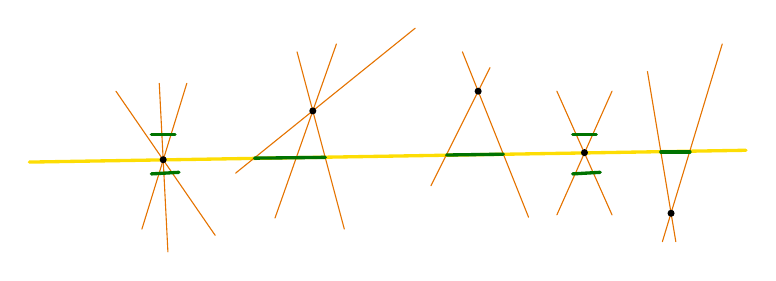
\begin{tikzpicture}[x=1mm,y=1mm,line cap=round,line join=round,font=\scriptsize]
\draw[Ye,very thick] (0,-21) -- (91,-19.5);
\draw[Or] (11,-12) -- (23.6,-30.3);
\draw[Or] (20,-11) -- (14.3,-29.5);
\draw[Or] (16.5,-11) -- (17.6,-32.4);
\draw[Dg,very thick] (15.5,-17.5) -- (18.5,-17.5);
\draw[Dg,very thick] (15.5,-22.5) -- (19,-22.3);
\node[pt] at (17,-20.7) {};
\draw[Or] (34,-7) -- (40,-29.5);
\draw[Or] (39,-6) -- (31.2,-28.1);
\draw[Or] (49,-4) -- (26.2,-22.4);
\node[pt] at (36,-14.5) {};
\draw[Dg,very thick] (28.6,-20.5) -- (37.6,-20.4);
\draw[Or] (55,-7) -- (63.4,-28);
\draw[Or] (58.5,-9) -- (51,-24);
\node[pt] at (57,-12) {};
\draw[Dg,very thick] (53,-20.1) -- (60.2,-20);
\draw[Or] (67,-12) -- (74,-27.7);
\draw[Or] (74,-12) -- (67,-27.7);
\node[pt] at (70.5,-19.8) {};
\draw[Dg,very thick] (69,-17.5) -- (72,-17.5);
\draw[Dg,very thick] (69,-22.5) -- (72.5,-22.3);
\draw[Or] (78.5,-9.5) -- (82.1,-31.1);
\draw[Or] (88,-6) -- (80.4,-31.1);
\node[pt] at (81.5,-27.5) {};
\draw[Dg,very thick] (80.2,-19.7) -- (83.9,-19.7);
\end{tikzpicture}
\end{document}
